%\VignetteIndexEntry{faoswsImputation: A package for the imputation of missing time series data in the Statistical Working System}
%\VignetteEngine{knitr::knitr}
\documentclass[nojss]{jss}
\usepackage{url}
\usepackage[sc]{mathpazo}
\usepackage{geometry}
\geometry{verbose,tmargin=2.5cm,bmargin=2.5cm,lmargin=2.5cm,rmargin=2.5cm}
\setcounter{secnumdepth}{2}
\setcounter{tocdepth}{2}
\usepackage{breakurl}
\usepackage{hyperref}
\usepackage[ruled, vlined]{algorithm2e}
\usepackage{mathtools}
\usepackage{draftwatermark}
\usepackage{float}
\usepackage{placeins}
\usepackage{mathrsfs}
\usepackage{multirow}
%% \usepackage{mathbbm}
\DeclareMathOperator{\sgn}{sgn}
\DeclareMathOperator*{\argmax}{\arg\!\max}

\title{\bf faoswsImputation: A package for the imputation of missing time
series data in the Statistical Working System}

\author{Joshua M. Browning\\ Food and Agriculture
    Organization \\ of the United Nations\\}

\Plainauthor{Joshua M. Browning}

\Plaintitle{faoswsImputation: A package for the imputation of missing time
series data in the Statistical Working System}

\Shorttitle{Ensemble Imputation}

\Abstract{ 

  This vignette provides a detailed description of the usage of
  functions in the \pkg{faoswsImputation} package. \\
  
}

\Keywords{Imputation, Linear Mixed Model, Ensemble Learning}
\Plainkeywords{Imputation, Linear Mixed Model, Ensemble Learning}

\Address{
  Joshua M. Browning\\
  Economics and Social Statistics Division (ESS)\\
  Economic and Social Development Department (ES)\\
  Food and Agriculture Organization of the United Nations (FAO)\\
  Viale delle Terme di Caracalla 00153 Rome, Italy\\
  E-mail: \email{joshua.browning@fao.org}\\
  URL: \url{https://svn.fao.org/projects/SWS/RModules/faoswsImputation/}
}

\begin{document}




\section{Setup}

Before we begin, we will need to load the required libraries

\begin{knitrout}
\definecolor{shadecolor}{rgb}{0.969, 0.969, 0.969}\color{fgcolor}\begin{kframe}
\begin{alltt}
\hlcom{## Load libraries}
\hlkwd{library}\hlstd{(faoswsImputation)}
\hlkwd{library}\hlstd{(faoswsUtil)}
\hlkwd{library}\hlstd{(data.table)}
\end{alltt}
\end{kframe}
\end{knitrout}

Additionally, we'll load the production library for an example dataset

\begin{knitrout}
\definecolor{shadecolor}{rgb}{0.969, 0.969, 0.969}\color{fgcolor}\begin{kframe}
\begin{alltt}
\hlkwd{library}\hlstd{(faoswsProduction)}
\end{alltt}
\end{kframe}
\end{knitrout}

To illustrate the functionality of the package, we take the Okra data
set as an example. The implementation requires the data to be loaded as
a \textit{data.table} object. This is also the default when data are
queried from the API of the Statistical Working System (SWS).

\begin{knitrout}
\definecolor{shadecolor}{rgb}{0.969, 0.969, 0.969}\color{fgcolor}\begin{kframe}
\begin{alltt}
\hlkwd{str}\hlstd{(okrapd)}
\end{alltt}
\begin{verbatim}
## Classes 'data.table' and 'data.frame':	836 obs. of  14 variables:
##  $ geographicAreaM49                         : int  3 3 3 3 3 3 3 3 3 3 ...
##  $ areaName                                  : chr  "Albania" "Albania" "Albania" "Albania" ...
##  $ itemCode                                  : int  430 430 430 430 430 430 430 430 430 430 ...
##  $ itemName                                  : chr  "Okra" "Okra" "Okra" "Okra" ...
##  $ timePointYears                            : int  1995 1996 1997 1998 1999 2000 2001 2002 2003 2004 ...
##  $ Value_measuredElement_5312                : num  800 600 750 750 740 780 790 780 700 600 ...
##  $ flagObservationStatus_measuredElement_5312: chr  "T" "T" "T" "T" ...
##  $ flagMethod_measuredElement_5312           : logi  NA NA NA NA NA NA ...
##  $ Value_measuredElement_5416                : num  7.25 8 8 8 7.97 ...
##  $ flagObservationStatus_measuredElement_5416: chr  "T" "T" "T" "T" ...
##  $ flagMethod_measuredElement_5416           : logi  NA NA NA NA NA NA ...
##  $ Value_measuredElement_5510                : num  5800 4800 6000 6000 5900 6200 6500 6700 6000 5300 ...
##  $ flagObservationStatus_measuredElement_5510: chr  "T" "T" "T" "T" ...
##  $ flagMethod_measuredElement_5510           : logi  NA NA NA NA NA NA ...
##  - attr(*, ".internal.selfref")=<externalptr>
\end{verbatim}
\end{kframe}
\end{knitrout}

Note: the okrapd dataset is a good example of the data available in the SWS.
However, as such, the column names aren't very clear.  As a quick explanation,
5312 refers to area harvested, 5416 refers to yield, and 5510 refers to
production.  Each variable has three columns for it's value and the two status
flags.

In addition to the data, the implementation also require a table to
map the hierachical relation of the observation flags. It
provides a rule for ``flag aggregation'' (the process of assigning a new
observation flag to an observation which is computed from other observations).
An example of the table is given below. For more details on flags and how to
create/interpret such tables, please see the vignette of the \pkg{faoswsFlag}
package.

%<<create-flagt-table, results='markup'>>=
\begin{knitrout}
\definecolor{shadecolor}{rgb}{0.969, 0.969, 0.969}\color{fgcolor}\begin{kframe}
\begin{alltt}
\hlstd{swsOldFlagTable} \hlkwb{=} \hlstd{faoswsFlagTable}
\hlstd{faoswsFlagTable}\hlopt{$}\hlstd{flagObservationStatus} \hlkwb{=}
    \hlkwd{as.character}\hlstd{(faoswsFlagTable}\hlopt{$}\hlstd{flagObservationStatus)}
\hlstd{swsOldFlagTable}
\end{alltt}
\begin{verbatim}
##   flagObservationStatus flagObservationWeights
## 1                                         1.00
## 2                     T                   0.80
## 3                     E                   0.75
## 4                     I                   0.50
## 5                     M                   0.00
\end{verbatim}
\end{kframe}
\end{knitrout}


\section{Functions}
This section describes the step-by-step usage of functions which are
used to perform imputation.  The steps/functions illustrated here are for
demonstration purposes only, as usually these functions will all be called by a
one-step imputation function \code{imputeProductionDomain} (i.e. a ``wrapper
function'').

\subsection{Data processing}

The first step of the imputation is to remove any previous imputations.
Even when using the same methodology and settings, prior
imputations will change as more information is received over time. This
step is highly recommended but optional and depends on the judgement
of the analyst. \\

To remove the prior imputations, one will need to specify the column
name of the value and corresponding observation and method flags.  Further,
the character value which represents an imputation and the character value
for a flag representing missing values must be provided. The function will
convert the previously imputed values to NA
and the flags from previous imputations will be set to the missing flag value.

\begin{knitrout}
\definecolor{shadecolor}{rgb}{0.969, 0.969, 0.969}\color{fgcolor}\begin{kframe}
\begin{alltt}
\hlstd{okraProcessed} \hlkwb{=} \hlkwd{copy}\hlstd{(okrapd)}

\hlcom{## Removing prior imputation for production}
\hlkwd{table}\hlstd{(okraProcessed}\hlopt{$}\hlstd{flagObservationStatus_measuredElement_5510)}
\end{alltt}
\begin{verbatim}
## 
##       M   T 
## 478 304  54
\end{verbatim}
\begin{alltt}
\hlkwd{removeImputation}\hlstd{(}\hlkwc{data} \hlstd{= okraProcessed,}
                 \hlkwc{value} \hlstd{=} \hlstr{"Value_measuredElement_5510"}\hlstd{,}
                 \hlkwc{observationFlag} \hlstd{=}
                     \hlstr{"flagObservationStatus_measuredElement_5510"}\hlstd{,}
                 \hlkwc{methodFlag} \hlstd{=} \hlstr{"flagMethod_measuredElement_5510"}\hlstd{,}
                 \hlkwc{imputedFlag} \hlstd{=} \hlstr{"E"}\hlstd{,}
                 \hlkwc{missingObservationFlag} \hlstd{=} \hlstr{"M"}\hlstd{,}
                 \hlkwc{missingMethodFlag} \hlstd{=} \hlstr{"u"}\hlstd{)}
\hlkwd{table}\hlstd{(okraProcessed}\hlopt{$}\hlstd{flagObservationStatus_measuredElement_5510)}
\end{alltt}
\begin{verbatim}
## 
##       M   T 
## 478 304  54
\end{verbatim}
\begin{alltt}
\hlcom{## Removing prior imputation for area harvested}
\hlkwd{table}\hlstd{(okraProcessed}\hlopt{$}\hlstd{flagObservationStatus_measuredElement_5312)}
\end{alltt}
\begin{verbatim}
## 
##       F   M   T 
## 411 173 190  62
\end{verbatim}
\begin{alltt}
\hlkwd{removeImputation}\hlstd{(}\hlkwc{data} \hlstd{= okraProcessed,}
                 \hlkwc{value} \hlstd{=} \hlstr{"Value_measuredElement_5312"}\hlstd{,}
                 \hlkwc{observationFlag} \hlstd{=}
                     \hlstr{"flagObservationStatus_measuredElement_5312"}\hlstd{,}
                 \hlkwc{methodFlag} \hlstd{=} \hlstr{"flagMethod_measuredElement_5312"}\hlstd{,}
                 \hlkwc{imputedFlag} \hlstd{=} \hlstr{"E"}\hlstd{,}
                 \hlkwc{missingObservationFlag} \hlstd{=} \hlstr{"M"}\hlstd{,}
                 \hlkwc{missingMethodFlag} \hlstd{=} \hlstr{"u"}\hlstd{)}
\hlkwd{table}\hlstd{(okraProcessed}\hlopt{$}\hlstd{flagObservationStatus_measuredElement_5312)}
\end{alltt}
\begin{verbatim}
## 
##       F   M   T 
## 411 173 190  62
\end{verbatim}
\begin{alltt}
\hlcom{## Removing prior imputation for yield}
\hlkwd{table}\hlstd{(okraProcessed}\hlopt{$}\hlstd{flagObservationStatus_measuredElement_5416)}
\end{alltt}
\begin{verbatim}
## 
##       M   T 
## 407 372  57
\end{verbatim}
\begin{alltt}
\hlkwd{removeImputation}\hlstd{(}\hlkwc{data} \hlstd{= okraProcessed,}
                 \hlkwc{value} \hlstd{=} \hlstr{"Value_measuredElement_5416"}\hlstd{,}
                 \hlkwc{observationFlag} \hlstd{=}
                     \hlstr{"flagObservationStatus_measuredElement_5416"}\hlstd{,}
                 \hlkwc{methodFlag} \hlstd{=} \hlstr{"flagMethod_measuredElement_5416"}\hlstd{,}
                 \hlkwc{imputedFlag} \hlstd{=} \hlstr{"E"}\hlstd{,}
                 \hlkwc{missingObservationFlag} \hlstd{=} \hlstr{"M"}\hlstd{,}
                 \hlkwc{missingMethodFlag} \hlstd{=} \hlstr{"u"}\hlstd{)}
\hlkwd{table}\hlstd{(okraProcessed}\hlopt{$}\hlstd{flagObservationStatus_measuredElement_5416)}
\end{alltt}
\begin{verbatim}
## 
##       M   T 
## 407 372  57
\end{verbatim}
\end{kframe}
\end{knitrout}

After removing prior imputations, the next step is to replace zero
values with a missing flag to values of NA. This is an issue from previous
data: some observations will be labeled as missing but given a value of zero
instead of a value of NA.

\begin{knitrout}
\definecolor{shadecolor}{rgb}{0.969, 0.969, 0.969}\color{fgcolor}\begin{kframe}
\begin{alltt}
\hlstd{okraProcessed[geographicAreaM49} \hlopt{==} \hlnum{12} \hlopt{&} \hlstd{timePointYears} \hlopt{>=} \hlnum{2005}\hlstd{,}
              \hlkwd{.}\hlstd{(Value_measuredElement_5312,}
                \hlstd{flagObservationStatus_measuredElement_5312)]}
\hlkwd{remove0M}\hlstd{(}\hlkwc{data} \hlstd{= okraProcessed,}
         \hlkwc{value} \hlstd{=} \hlstr{"Value_measuredElement_5312"}\hlstd{,}
         \hlkwc{flag} \hlstd{=} \hlstr{"flagObservationStatus_measuredElement_5312"}\hlstd{,}
         \hlkwc{naFlag} \hlstd{=} \hlstr{"M"}\hlstd{)}
\hlstd{okraProcessed[geographicAreaM49} \hlopt{==} \hlnum{12} \hlopt{&} \hlstd{timePointYears} \hlopt{>=} \hlnum{2005}\hlstd{,}
              \hlkwd{.}\hlstd{(Value_measuredElement_5312,}
                \hlstd{flagObservationStatus_measuredElement_5312)]}
\end{alltt}
\begin{verbatim}
##    Value_measuredElement_5312 flagObservationStatus_measuredElement_5312
## 1:                         NA                                          M
## 2:                         NA                                          M
## 3:                         NA                                          M
## 4:                         NA                                          M
## 5:                         NA                                          M
## 6:                         19                                           
## 7:                         19                                           
## 8:                         19                                           
## 9:                         19                                          T
\end{verbatim}
\end{kframe}
\end{knitrout}

Note how the zeroes have been changed into NA's above.  Let's do the same for
production and area harvested:

\begin{knitrout}
\definecolor{shadecolor}{rgb}{0.969, 0.969, 0.969}\color{fgcolor}\begin{kframe}
\begin{alltt}
\hlkwd{remove0M}\hlstd{(}\hlkwc{data} \hlstd{= okraProcessed,}
         \hlkwc{value} \hlstd{=} \hlstr{"Value_measuredElement_5416"}\hlstd{,}
         \hlkwc{flag} \hlstd{=} \hlstr{"flagObservationStatus_measuredElement_5416"}\hlstd{,}
         \hlkwc{naFlag} \hlstd{=} \hlstr{"M"}\hlstd{)}

\hlkwd{remove0M}\hlstd{(}\hlkwc{data} \hlstd{= okraProcessed,}
         \hlkwc{value} \hlstd{=} \hlstr{"Value_measuredElement_5510"}\hlstd{,}
         \hlkwc{flag} \hlstd{=} \hlstr{"flagObservationStatus_measuredElement_5510"}\hlstd{,}
         \hlkwc{naFlag} \hlstd{=} \hlstr{"M"}\hlstd{)}
\end{alltt}
\end{kframe}
\end{knitrout}


In order for the linear mixed model (one of the models in the ensemble that
we will later fit) to fit successfully, at least one
observation is required for each country. Thus, this function removes
countries which contain no non-missing observations.

\begin{knitrout}
\definecolor{shadecolor}{rgb}{0.969, 0.969, 0.969}\color{fgcolor}\begin{kframe}
\begin{alltt}
\hlstd{okraProcessed[geographicAreaM49} \hlopt{==} \hlnum{245}\hlstd{,}
              \hlkwd{.}\hlstd{(Value_measuredElement_5416,}
                \hlstd{flagObservationStatus_measuredElement_5416)]}
\end{alltt}
\begin{verbatim}
## Empty data.table (0 rows) of 2 cols: Value_measuredElement_5416,flagObservationStatus_measuredElement_5416
\end{verbatim}
\begin{alltt}
\hlkwd{removeNoInfo}\hlstd{(}\hlkwc{data} \hlstd{= okraProcessed,}
             \hlkwc{value} \hlstd{=} \hlstr{"Value_measuredElement_5416"}\hlstd{,}
             \hlkwc{observationFlag} \hlstd{=} \hlstr{"flagObservationStatus_measuredElement_5416"}\hlstd{,}
             \hlkwc{byKey} \hlstd{=} \hlstr{"geographicAreaM49"}\hlstd{)}
\hlstd{okraProcessed[geographicAreaM49} \hlopt{==} \hlnum{245}\hlstd{,}
              \hlkwd{.}\hlstd{(Value_measuredElement_5416,}
                \hlstd{flagObservationStatus_measuredElement_5416)]}
\end{alltt}
\begin{verbatim}
## Empty data.table (0 rows) of 2 cols: Value_measuredElement_5416,flagObservationStatus_measuredElement_5416
\end{verbatim}
\end{kframe}
\end{knitrout}

Note for advanced users: All other remove* functions from the utils package
perform by modifying the data.table in place (and thus you do not need to
assign a new data.table to the result of a function).  removeNoInfo should work
in the same way, but there is currently not a way to delete rows in a
data.table without copying the data.table.  Thus, the object cannot be modified
in place.  For this function to behave like the other functions, then, we
assign the data.table object in an environment (by default, the calling
environment of removeNoInfo).  This should be changed once the \pkg{data.table}
package adds this functionality.

Next, we must create a list that contains specific parameters on how the
processing should be performed.

\begin{knitrout}
\definecolor{shadecolor}{rgb}{0.969, 0.969, 0.969}\color{fgcolor}\begin{kframe}
\begin{alltt}
\hlstd{processingParams} \hlkwb{=} \hlkwd{defaultProcessingParameters}\hlstd{()}
\hlstd{processingParams}
\end{alltt}
\begin{verbatim}
## $productionValue
## [1] "Value_measuredElement_5510"
## 
## $productionObservationFlag
## [1] "flagObservationStatus_measuredElement_5510"
## 
## $productionMethodFlag
## [1] "flagMethod_measuredElement_5510"
## 
## $yieldValue
## [1] "Value_measuredElement_5416"
## 
## $yieldObservationFlag
## [1] "flagObservationStatus_measuredElement_5416"
## 
## $yieldMethodFlag
## [1] "flagMethod_measuredElement_5416"
## 
## $areaHarvestedValue
## [1] "Value_measuredElement_5312"
## 
## $areaHarvestedObservationFlag
## [1] "flagObservationStatus_measuredElement_5312"
## 
## $areaHarvestedMethodFlag
## [1] "flagMethod_measuredElement_5312"
## 
## $yearValue
## [1] "timePointYears"
## 
## $byKey
## [1] "geographicAreaM49"
## 
## $removePriorImputation
## [1] TRUE
## 
## $removeConflictValues
## [1] TRUE
## 
## $imputedFlag
## [1] "E"
## 
## $naFlag
## [1] "M"
\end{verbatim}
\end{kframe}
\end{knitrout}

Now, we will pass processingParams through all of the individual processing
functions.  The function \code{processProductionDomain} is a wrapper that
executes all the data processing above.

\begin{knitrout}
\definecolor{shadecolor}{rgb}{0.969, 0.969, 0.969}\color{fgcolor}\begin{kframe}
\begin{alltt}
\hlstd{okraProcessed} \hlkwb{=} \hlkwd{copy}\hlstd{(okrapd)}
\hlkwd{processProductionDomain}\hlstd{(}\hlkwc{data} \hlstd{= okraProcessed,}
                        \hlkwc{processingParameters} \hlstd{= processingParams)}
\end{alltt}
\end{kframe}
\end{knitrout}

\subsection{Imputation}

Now we are ready to perform the imputation.  First, we'll impute the yield.
The function \code{imputeVariable}
allows the user to perform imputation on the dataset, and it accepts
a list of imputation parameters which control how the imputation is done.

To run the imputation, we need to construct a list with the default imputation
parameters (similar to the list with the processing parameters) and adjust
them as necessary for our specific use case.  The
documentation page for defaultImputationParameters() provides some detail on
what each of the different elements of this list are.  Also, let's delete some
of the data (having too many countries can clog up some of the later plots).

\begin{knitrout}
\definecolor{shadecolor}{rgb}{0.969, 0.969, 0.969}\color{fgcolor}\begin{kframe}
\begin{alltt}
\hlstd{okraProcessed} \hlkwb{=} \hlstd{okraProcessed[geographicAreaM49} \hlopt{<=} \hlnum{60}\hlstd{, ]}
\hlstd{imputationParams} \hlkwb{=} \hlkwd{defaultImputationParameters}\hlstd{(}\hlkwc{variable} \hlstd{=} \hlstr{"yield"}\hlstd{)}
\hlkwd{sapply}\hlstd{(imputationParams, class)}
\end{alltt}
\begin{verbatim}
##              yearValue                  byKey         ensembleModels 
##            "character"            "character"                 "list" 
##        restrictWeights         maximumWeights         plotImputation 
##              "logical"              "numeric"              "logical" 
##              errorType          errorFunction             groupCount 
##            "character"             "function"              "numeric" 
##            missingFlag         imputationFlag          newMethodFlag 
##            "character"            "character"            "character" 
##              flagTable               variable  imputationValueColumn 
##           "data.frame"            "character"            "character" 
##   imputationFlagColumn imputationMethodColumn    newImputationColumn 
##            "character"            "character"            "character" 
##         estimateNoData 
##              "logical"
\end{verbatim}
\end{kframe}
\end{knitrout}

One very important part of this list is the ensembleModels element.  This
element specifies all of the models which should be used to form the final
ensemble.  By default, ten models are used.  However, let's use a simpler
example with just three models:

\begin{knitrout}
\definecolor{shadecolor}{rgb}{0.969, 0.969, 0.969}\color{fgcolor}\begin{kframe}
\begin{alltt}
\hlkwd{names}\hlstd{(imputationParams}\hlopt{$}\hlstd{ensembleModels)}
\end{alltt}
\begin{verbatim}
##  [1] "defaultMean"       "defaultLm"         "defaultExp"       
##  [4] "defaultLogistic"   "defaultLoess"      "defaultSpline"    
##  [7] "defaultArima"      "defaultMars"       "defaultNaive"     
## [10] "defaultMixedModel"
\end{verbatim}
\begin{alltt}
\hlstd{imputationParams}\hlopt{$}\hlstd{ensembleModels} \hlkwb{=}
    \hlstd{imputationParams}\hlopt{$}\hlstd{ensembleModels[}\hlnum{1}\hlopt{:}\hlnum{3}\hlstd{]}
\hlkwd{names}\hlstd{(imputationParams}\hlopt{$}\hlstd{ensembleModels)}
\end{alltt}
\begin{verbatim}
## [1] "defaultMean" "defaultLm"   "defaultExp"
\end{verbatim}
\end{kframe}
\end{knitrout}

You can also manually create your own model for use.  See the documentation
page for ?ensembleModel for more details, and below for an example:

\begin{knitrout}
\definecolor{shadecolor}{rgb}{0.969, 0.969, 0.969}\color{fgcolor}\begin{kframe}
\begin{alltt}
\hlstd{newModel} \hlkwb{=} \hlkwd{ensembleModel}\hlstd{(}
    \hlkwc{model} \hlstd{=} \hlkwa{function}\hlstd{(}\hlkwc{data}\hlstd{)\{}
        \hlkwd{rep}\hlstd{(}\hlnum{10}\hlstd{,} \hlkwd{length}\hlstd{(data))}
    \hlstd{\},}
    \hlkwc{extrapolationRange} \hlstd{=} \hlnum{5}\hlstd{,}
    \hlkwc{level} \hlstd{=} \hlstr{"countryCommodity"}\hlstd{)}
\hlkwd{is}\hlstd{(newModel)}
\end{alltt}
\begin{verbatim}
## [1] "ensembleModel"
\end{verbatim}
\begin{alltt}
\hlstd{imputationParams}\hlopt{$}\hlstd{ensembleModels} \hlkwb{=} \hlkwd{c}\hlstd{(imputationParams}\hlopt{$}\hlstd{ensembleModels,}
                                    \hlkwc{newModel} \hlstd{= newModel)}
\hlkwd{names}\hlstd{(imputationParams}\hlopt{$}\hlstd{ensembleModels)}
\end{alltt}
\begin{verbatim}
## [1] "defaultMean" "defaultLm"   "defaultExp"  "newModel"
\end{verbatim}
\end{kframe}
\end{knitrout}

This new model returns a constant prediction of 10.  It's not a good model,
but it's a simple example of how to create a new model.  The extrapolation
range specifies that the model can be used in an ensemble up to 5 observations
outside the range of the data, but no more.  The level argument specifies that
the model should operate on data for all countries for a fixed commodity (as
opposed to one model for each unique country-commodity pair).

\begin{knitrout}
\definecolor{shadecolor}{rgb}{0.969, 0.969, 0.969}\color{fgcolor}\begin{kframe}
\begin{alltt}
\hlstd{imputationParams}\hlopt{$}\hlstd{newImputationColumn} \hlkwb{=} \hlstr{"test"}
\hlkwd{imputeVariable}\hlstd{(}\hlkwc{data} \hlstd{= okraProcessed,} \hlkwc{imputationParameters} \hlstd{= imputationParams)}
\hlkwd{colnames}\hlstd{(okraProcessed)}
\end{alltt}
\begin{verbatim}
##  [1] "geographicAreaM49"                         
##  [2] "areaName"                                  
##  [3] "itemCode"                                  
##  [4] "itemName"                                  
##  [5] "timePointYears"                            
##  [6] "Value_measuredElement_5312"                
##  [7] "flagObservationStatus_measuredElement_5312"
##  [8] "flagMethod_measuredElement_5312"           
##  [9] "Value_measuredElement_5416"                
## [10] "flagObservationStatus_measuredElement_5416"
## [11] "flagMethod_measuredElement_5416"           
## [12] "Value_measuredElement_5510"                
## [13] "flagObservationStatus_measuredElement_5510"
## [14] "flagMethod_measuredElement_5510"           
## [15] "Value_test"                                
## [16] "flagObservationStatus_test"                
## [17] "flagMethod_test"
\end{verbatim}
\end{kframe}

{\centering 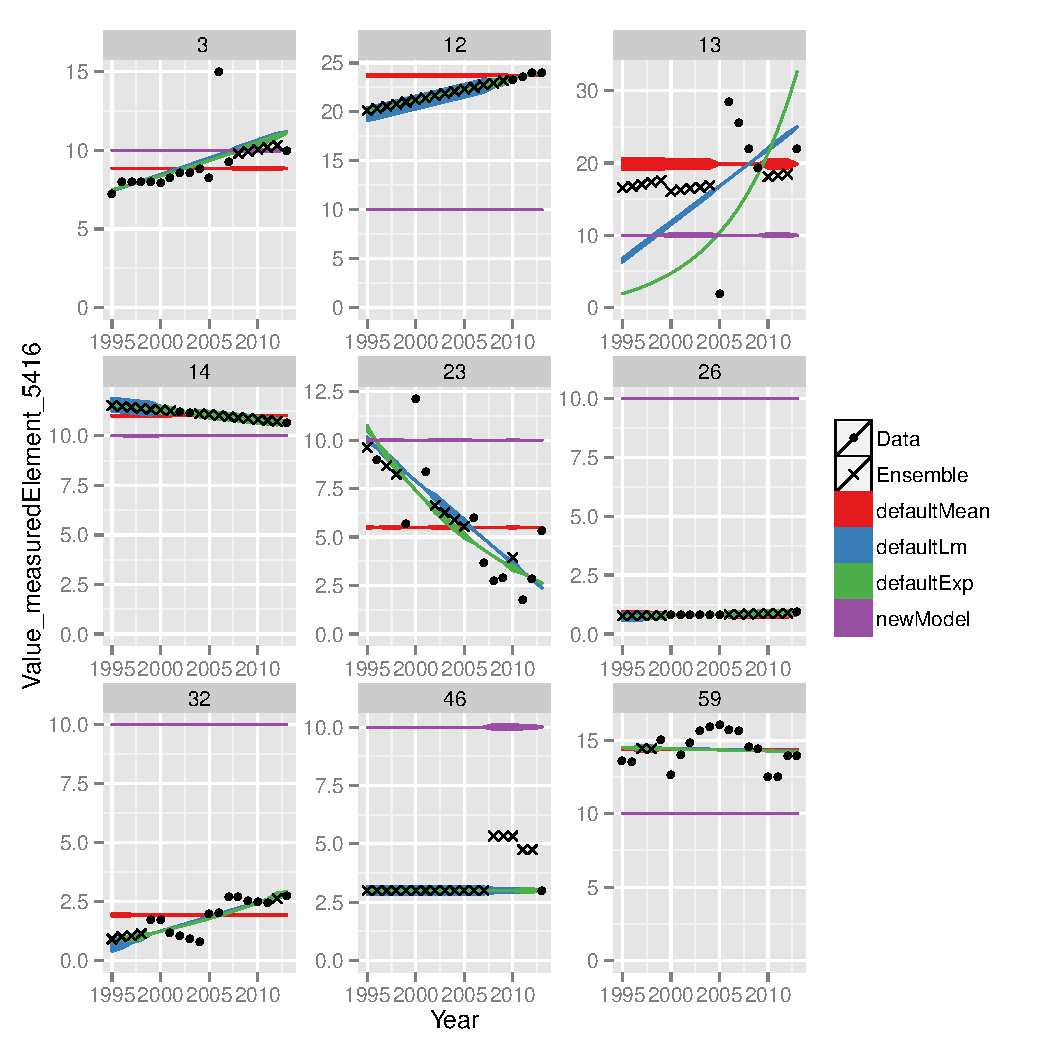
\includegraphics[width=\maxwidth]{figure/impute-yield-1} 

}



\end{knitrout}

Before discussing the output, first note that the newImputationColumn parameter
was updated in the imputationParams object.  This parameter allows you to store
the imputations from the model in three new columns (value, observation flag,
and method flag).  This allows you to examine several different ensembles and
compare their performances.  The default value of
imputationParams\$newImputationColumn is just an empty string, and in this case
the imputation will place the imputations into the processed data.table.

The graphs contain a lot of information.  First, the dots represent observed
values, and the crosses represent the imputations.  The different colored lines
show the different fits, and the thickness of the line is proportional to the
weight it received in the ensemble.  Of course, if the data point is an
observation then no imputation is done, so all lines have the same thickness
there.  Also, the computed weights will be constant for all imputed values with
one exception: models that are not allowed to extrapolate may have positive
weights for some imputations and 0 for others.  Moreover, if an observation
is outside the extrapolation range of a model, then the weight of all other
models will need to be rescaled so all values add to 1.

We see that the purple line (the model corresponding to our naive model which
always estimates the value 10) rarely gets any weight.  This makes sense, as
it's not a very good model.  However, in some particular cases (i.e.
geographicAreaM49 = 13), no models do very well.  The mean model thus gets most
of the weight, but our naive model also gets a little weight.  You can also see
how it only has weight up to 5 observations outside of the range of the data;
this is because we gave the model an extrapolation range of 5.

Now, suppose we wanted to remove the naive model which always predicts 10.  We
can do that and re-examine what our ensemble looks like:

\begin{knitrout}
\definecolor{shadecolor}{rgb}{0.969, 0.969, 0.969}\color{fgcolor}\begin{kframe}
\begin{alltt}
\hlstd{imputationParams}\hlopt{$}\hlstd{ensembleModels} \hlkwb{=} \hlstd{imputationParams}\hlopt{$}\hlstd{ensembleModels[}\hlopt{-}\hlnum{4}\hlstd{]}
\hlkwd{names}\hlstd{(imputationParams}\hlopt{$}\hlstd{ensembleModels)}
\end{alltt}
\begin{verbatim}
## [1] "defaultMean" "defaultLm"   "defaultExp"
\end{verbatim}
\begin{alltt}
\hlkwd{imputeVariable}\hlstd{(}\hlkwc{data} \hlstd{= okraProcessed,} \hlkwc{imputationParameters} \hlstd{= imputationParams)}
\end{alltt}
\end{kframe}

{\centering 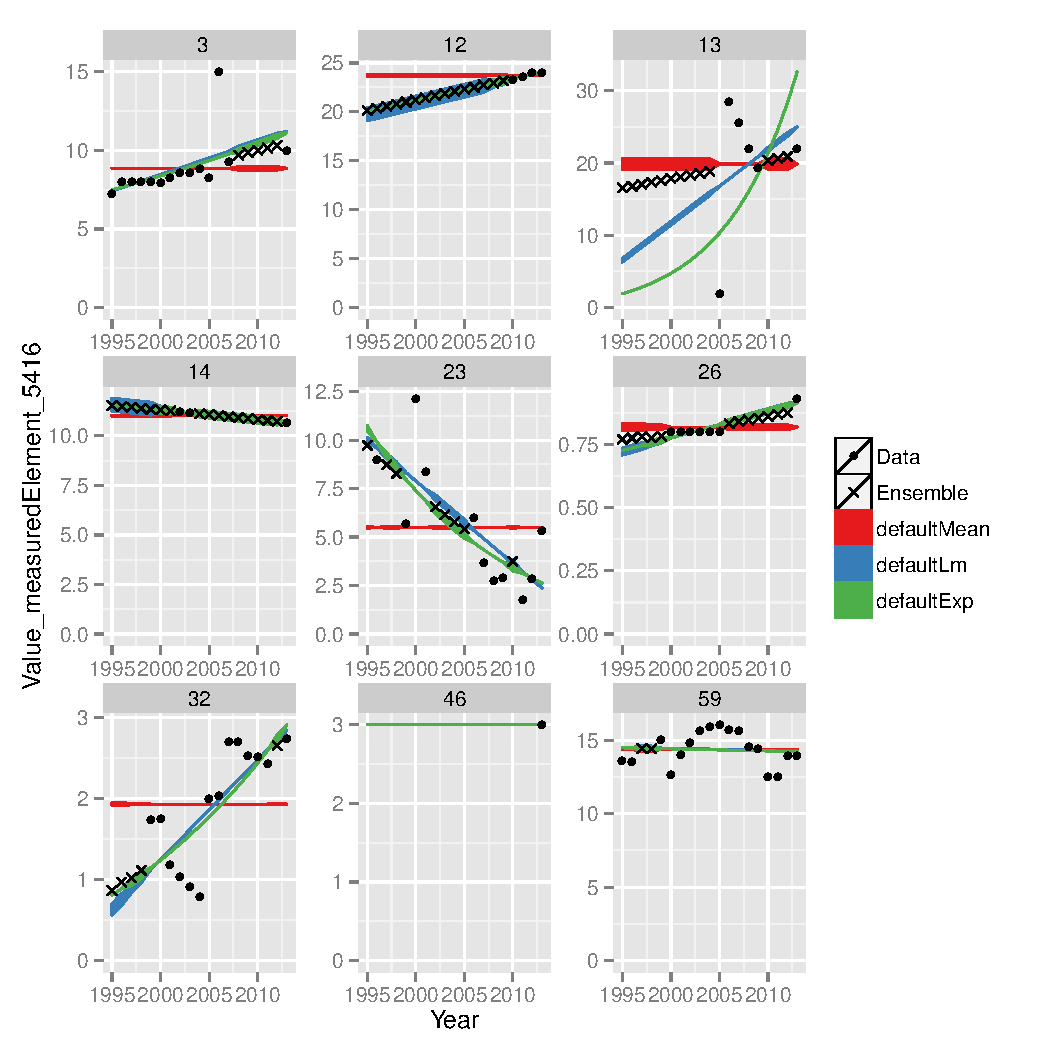
\includegraphics[width=\maxwidth]{figure/unnamed-chunk-3-1} 

}



\end{knitrout}

If we're happy with this model, we can assign these imputed values back to the
original variable:

\begin{knitrout}
\definecolor{shadecolor}{rgb}{0.969, 0.969, 0.969}\color{fgcolor}\begin{kframe}
\begin{alltt}
\hlstd{imputationParams}\hlopt{$}\hlstd{newImputationColumn} \hlkwb{=} \hlstr{""}
\hlkwd{imputeVariable}\hlstd{(}\hlkwc{data} \hlstd{= okraProcessed,} \hlkwc{imputationParameters} \hlstd{= imputationParams)}
\hlstd{okraProcessed[,} \hlkwd{c}\hlstd{(}\hlstr{"Value_test"}\hlstd{,} \hlstr{"flagObservationStatus_test"}\hlstd{,}
                  \hlstr{"flagMethod_test"}\hlstd{)} \hlkwb{:=} \hlkwa{NULL}\hlstd{]}
\end{alltt}
\begin{verbatim}
##      geographicAreaM49 areaName itemCode itemName timePointYears
##   1:                 3  Albania      430     Okra           1995
##   2:                 3  Albania      430     Okra           1996
##   3:                 3  Albania      430     Okra           1997
##   4:                 3  Albania      430     Okra           1998
##   5:                 3  Albania      430     Okra           1999
##  ---                                                            
## 205:                59    Egypt      430     Okra           2009
## 206:                59    Egypt      430     Okra           2010
## 207:                59    Egypt      430     Okra           2011
## 208:                59    Egypt      430     Okra           2012
## 209:                59    Egypt      430     Okra           2013
##      Value_measuredElement_5312 flagObservationStatus_measuredElement_5312
##   1:                        800                                          T
##   2:                        600                                          T
##   3:                        750                                          T
##   4:                        750                                          T
##   5:                        740                                          T
##  ---                                                                      
## 205:                       9325                                           
## 206:                       6885                                           
## 207:                       6725                                           
## 208:                       6957                                           
## 209:                       6957                                          T
##      flagMethod_measuredElement_5312 Value_measuredElement_5416
##   1:                              NA                   7.250000
##   2:                              NA                   8.000000
##   3:                              NA                   8.000000
##   4:                              NA                   8.000000
##   5:                              NA                   7.972973
##  ---                                                           
## 205:                              NA                  14.441287
## 206:                              NA                  12.524619
## 207:                              NA                  12.496803
## 208:                              NA                  13.958315
## 209:                              NA                  13.958315
##      flagObservationStatus_measuredElement_5416 flagMethod_measuredElement_5416
##   1:                                          T                              NA
##   2:                                          T                              NA
##   3:                                          T                              NA
##   4:                                          T                              NA
##   5:                                          T                              NA
##  ---                                                                           
## 205:                                                                         NA
## 206:                                                                         NA
## 207:                                                                         NA
## 208:                                                                         NA
## 209:                                          T                              NA
##      Value_measuredElement_5510 flagObservationStatus_measuredElement_5510
##   1:                       5800                                          T
##   2:                       4800                                          T
##   3:                       6000                                          T
##   4:                       6000                                          T
##   5:                       5900                                          T
##  ---                                                                      
## 205:                     134665                                           
## 206:                      86232                                           
## 207:                      84041                                           
## 208:                      97108                                           
## 209:                      97108                                          T
##      flagMethod_measuredElement_5510
##   1:                              NA
##   2:                              NA
##   3:                              NA
##   4:                              NA
##   5:                              NA
##  ---                                
## 205:                              NA
## 206:                              NA
## 207:                              NA
## 208:                              NA
## 209:                              NA
\end{verbatim}
\end{kframe}

{\centering 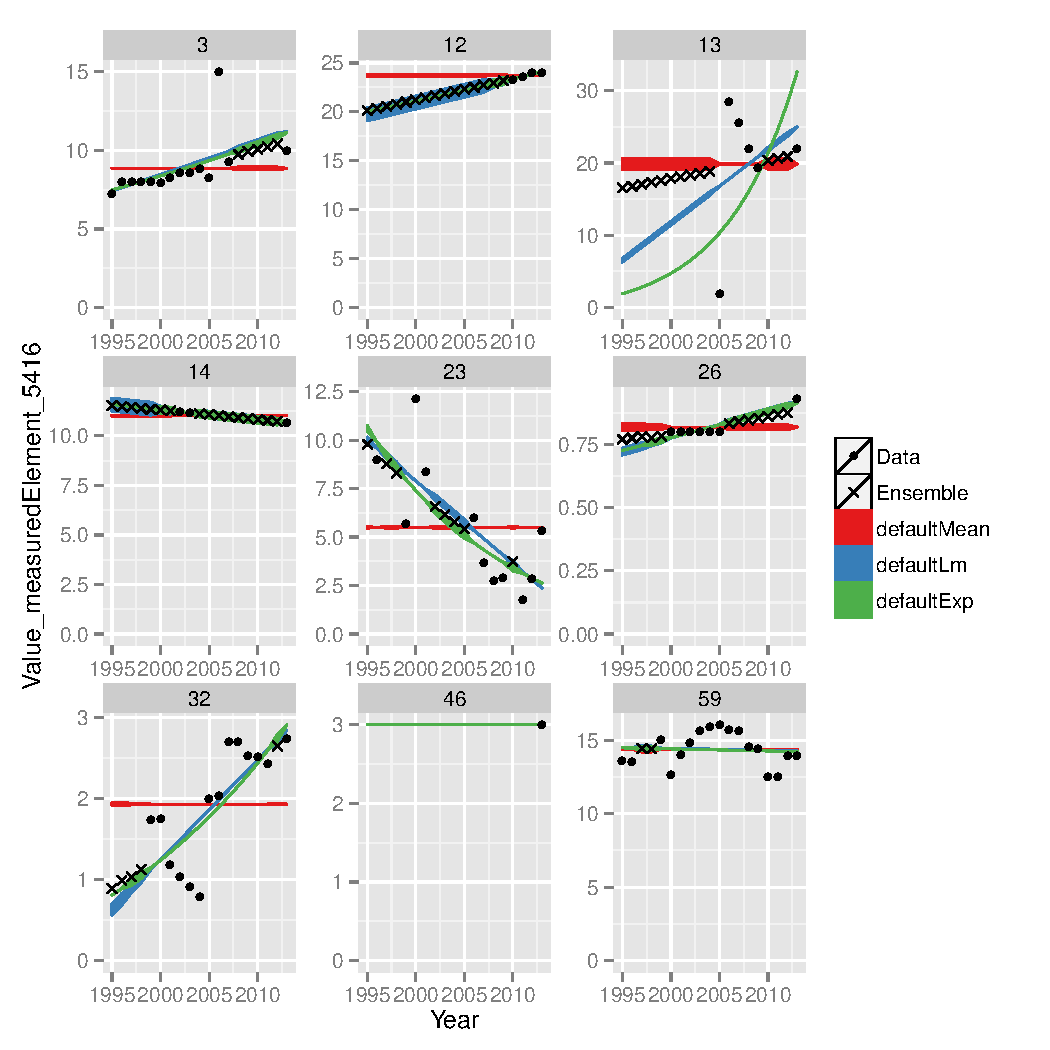
\includegraphics[width=\maxwidth]{figure/unnamed-chunk-4-1} 

}



\end{knitrout}

If we now try to impute again, we see that imputation fails because we have no
missing observations.  Well, to be more accurate, we have missing observations
in one country with only one valid observation.  This country was not
possible to impute because no leave-one-out cross-validation error can be
calculated with a single observation and thus no ensemble weights can be
choosen.

\begin{knitrout}
\definecolor{shadecolor}{rgb}{0.969, 0.969, 0.969}\color{fgcolor}\begin{kframe}
\begin{alltt}
\hlkwd{imputeVariable}\hlstd{(}\hlkwc{data} \hlstd{= okraProcessed,} \hlkwc{imputationParameters} \hlstd{= imputationParams)}
\end{alltt}
\end{kframe}

{\centering 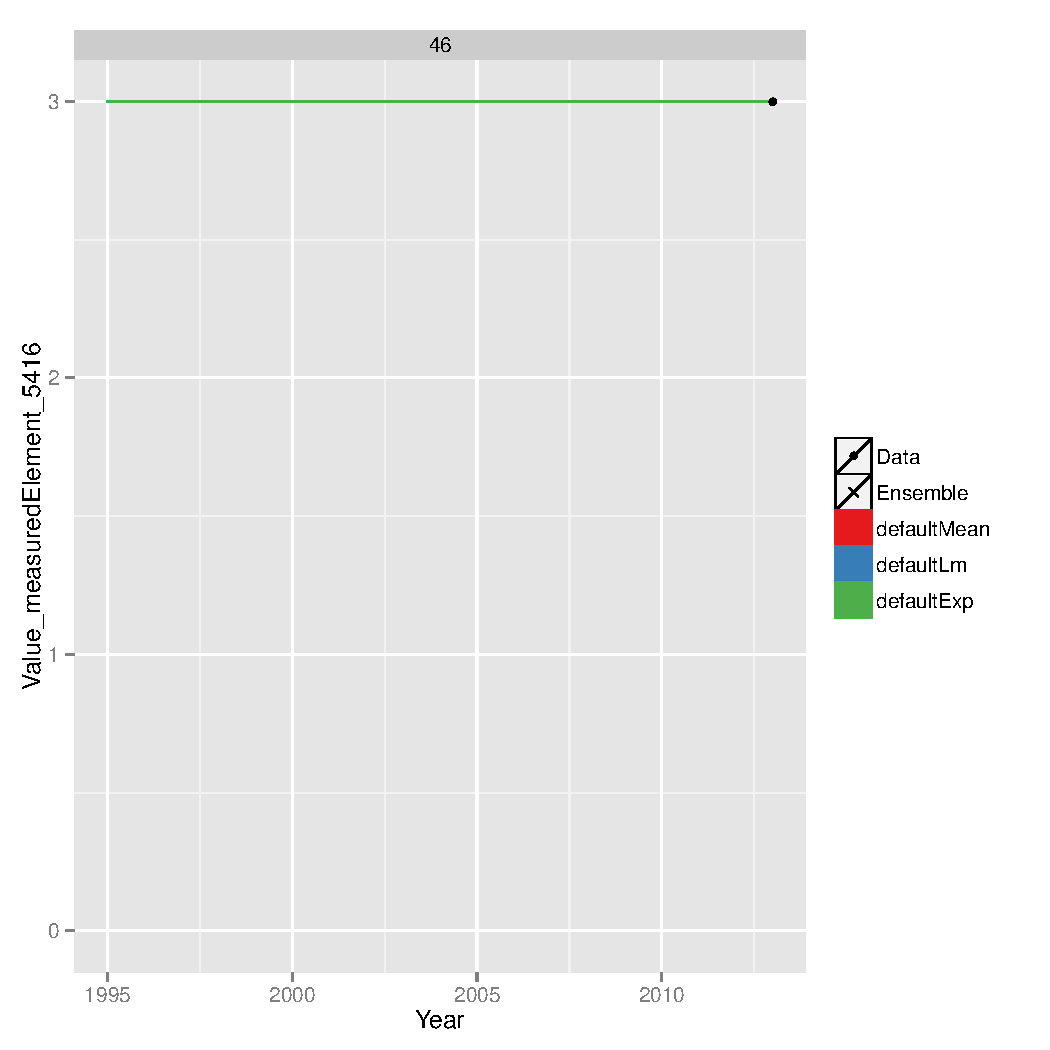
\includegraphics[width=\maxwidth]{figure/unnamed-chunk-5-1} 

}



\end{knitrout}

After the imputation of yield, we proceed to impute the production.  The
function \code{imputeVariable} is used again, but we first need to impute
by ``balancing,'' i.e. updating missing values of production when yield and
area harvested both exist.  This is because we have the relationship:
$$Y = P / A$$
where $Y$ is yield, $P$ is production, and $A$ is the area harvested.
If no value for area harvested is available, then the function proceeds to
impute the remaining production values with ensemble learning.  Let's use
some different models this time, just for the purpose of showing what's
available.

























































